\chapter{Unified Multimodal Binding for Joint Zero-Shot Camera Trap Understanding}\label{cap:experiment_03}

The previous two chapters established two complementary but partial findings. Chapter~\ref{cap:experiment_01} showed that pre-trained multimodal models can support empty-image filtering, species classification, and behavior identification, but that no single model, supervision regime, or input context is uniformly superior across the three tasks: each task was evaluated with its own prompts, its own candidate label set, and its own scoring pipeline. Chapter~\ref{cap:experiment_02} showed that explicitly combining two complementary zero-shot signals---CLIP-based visual similarity and language-model-generated textual similarity---can improve species classification over either signal alone, but the fusion mechanism was a single global weight ($\alpha=0.7$) tuned by hand, applied to exactly two evidence sources, and restricted to one task.

This chapter proposes and specifies WildBind, a unified multimodal binding architecture intended to close the gap between these two findings. Rather than treating empty-image filtering, species classification, and behavior identification as three independently engineered pipelines, WildBind represents all three as retrieval problems over a single shared \textit{Ecological Ontology Graph} embedded in a common latent space. Rather than combining two evidence sources with a fixed linear weight, WildBind learns a compact, uncertainty-aware gating function that adaptively weighs an arbitrary number of visual, textual, temporal, and sequence-level evidence sources, and that degrades gracefully when any of them is unavailable. The remainder of this chapter motivates the design, specifies the architecture and training procedure, and details the planned experimental evaluation, including datasets, baselines, metrics, and statistical tests.

\section{Introduction}

\subsection{Motivation}

The multi-task evaluation in Chapter~\ref{cap:experiment_01} and the fusion study in Chapter~\ref{cap:experiment_02} converge on the same diagnosis: standalone multimodal inference is unstable across models, tasks, and classes, and even an explicit two-branch fusion strategy only partially stabilizes this behavior, because it is task-specific, uses a fixed combination weight, and requires both evidence sources to be present for every instance. At the same time, the literature reviewed in Chapter~\ref{cap:related_work} shows a second, related gap: general-purpose unified vision-language systems for camera traps, exemplified by CameraTrap-Instruct \citep{chen2026cameratrap}, achieve strong multi-task performance (species identification, counting, and behavior classification from a single instruction-tuned model) but do so by fine-tuning a large vision-language backbone (Qwen2.5-VL-7B-Instruct with LoRA adapters) on an attribute-rich, manually curated instruction dataset. This reintroduces exactly the dependency on large annotated, task-specific data that motivates the low-supervision perspective of this thesis (Hypotheses H1--H3, Chapter~\ref{cap:introduction}).

This chapter is motivated by a design question that neither of the previous two chapters nor CameraTrap-Instruct directly answers: \textit{can multiple heterogeneous ecological evidence sources be integrated into a single learned representation, jointly covering the three camera-trap tasks, without sacrificing the zero-shot, low-supervision character of the overall thesis, and without requiring every evidence source to be present at inference time?}

\subsection{Inspiration from Multimodal Binding Outside Ecology}

A structurally similar problem has recently been addressed outside biodiversity monitoring, in the prediction of protein function from heterogeneous biological modalities. Boadu et al. \citep{boadu2025funbind} propose FunBind, a multimodal model that aligns protein sequence, structure, textual description, and domain-annotation embeddings in a single contrastively learned latent space, using the sequence modality as a central anchor because it is the only modality guaranteed to be available for every protein. After self-supervised contrastive pretraining, FunBind supports two complementary prediction regimes from the same backbone: an unsupervised zero-shot regime, in which a candidate functional term is scored purely by embedding similarity to the anchor modality, and a supervised regime, in which lightweight classification heads are fine-tuned on top of the frozen, aligned representations and their per-modality predictions are fused by weighted averaging. Crucially, because every non-anchor modality is optional, the model tolerates missing modalities at both training and inference time, and the fusion weights are optimized on held-out data rather than fixed by hand.

WildBind adapts this design principle to the camera-trap domain. The role of the protein sequence as an always-available anchor is played by the visual embedding of the event's most informative frame. The role of structure, text, and domain annotations is played by burst-level visual context, generated image descriptions, species/behavior knowledge-base text, and spatiotemporal metadata; and the role of Gene Ontology terms as the open-ended prediction target is played by a hierarchical Ecological Ontology Graph that spans all three tasks investigated in this thesis. The analogy is not exact---camera-trap events are not proteins, and ecological semantics are far less standardized than Gene Ontology---but the underlying architectural principle (anchor-centered contrastive binding, optional peripheral modalities, and a fusion step that is learned rather than fixed) transfers directly and addresses precisely the three structural gaps identified above.

\subsection{Positioning Relative to Chapters~\ref{cap:experiment_01} and~\ref{cap:experiment_02}, and to CameraTrap-Instruct}

WildBind is not a simple extension of WildMatch-VLM-Fusion to more modalities, nor a re-implementation of CameraTrap-Instruct without fine-tuning. Three design decisions distinguish it from both:

\begin{enumerate}
\item \textbf{Task unification through a shared ontology, not a shared prompt.} Chapter~\ref{cap:experiment_01} used a different prompt and candidate set for each task. CameraTrap-Instruct uses a single model but produces task outputs through separate instruction-tuned generation heads/formats. WildBind instead defines one hierarchical label space (presence, species, behavior) whose nodes are all embedded through the same textual encoder into the same latent space as the visual evidence, so that empty-image filtering, species classification, and behavior identification become the same operation---nearest-neighbor retrieval over ontology nodes---executed at different levels of a hierarchy.
\item \textbf{Learned, uncertainty-aware fusion instead of a fixed weight or an implicit one.} Chapter~\ref{cap:experiment_02} fixed $\alpha=0.7$ for every instance. WildBind replaces this constant with a small gating network trained on held-out data, whose inputs include per-modality confidence statistics (probability margin and normalized entropy of each modality's own ranking, computed directly from the similarity scores as detailed in Section~\ref{sec:fusion_gate}) and a binary modality-availability mask.
\item \textbf{Preserving low-supervision by keeping the backbones frozen.} Unlike CameraTrap-Instruct, WildBind does not fine-tune a large vision-language model end to end. The visual and textual base encoders remain frozen. Only lightweight projection heads and the fusion gate are trained, using orders of magnitude fewer parameters and far smaller labeled subsets (the validation partitions already produced in Chapters~\ref{cap:experiment_01} and~\ref{cap:experiment_02}) than an instruction-tuning pipeline would require. This keeps the contribution consistent with the general objective of the thesis: reducing, not reintroducing, dependence on large task-specific annotated datasets.
\end{enumerate}

\section{Proposed Architecture: WildBind}

\begin{figure*}[!ht]
\centering
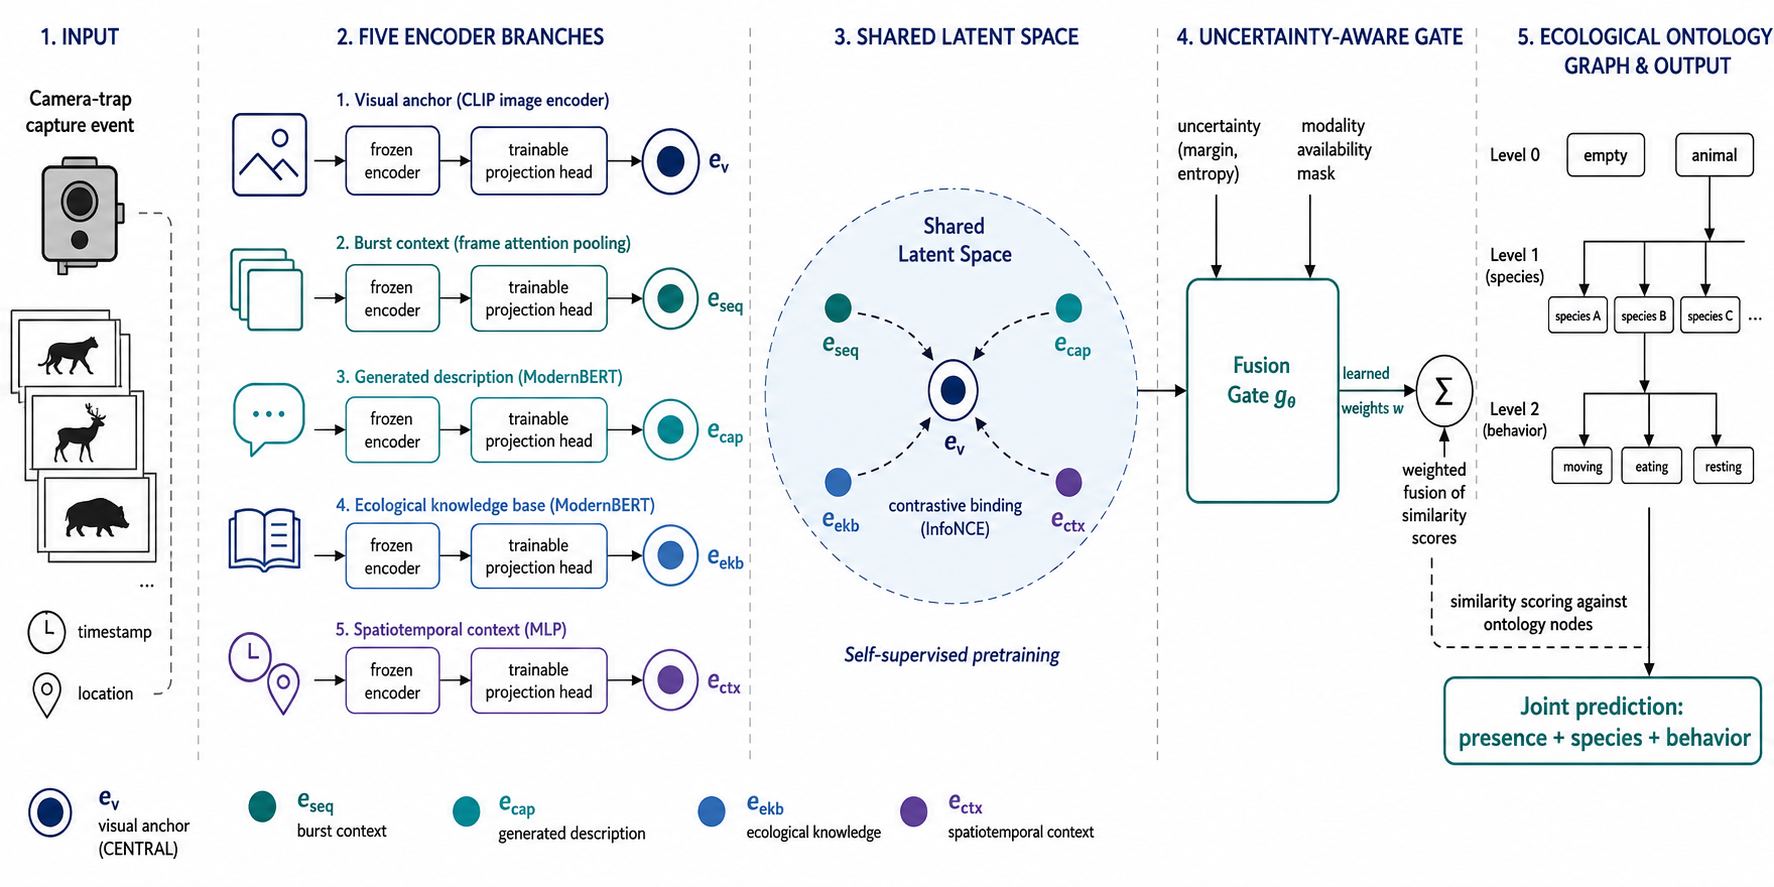
\includegraphics[width=6in]{images/wildbind_pipeline.png}
\caption{Overview of the WildBind architecture. A visual anchor embedding is contrastively bound to four peripheral modalities during self-supervised pretraining. At inference time, an uncertainty-aware gate fuses the available modality-specific similarity scores against the nodes of the Ecological Ontology Graph, producing a joint presence/species/behavior prediction.}
\label{fig:wildbind_pipeline}
\end{figure*}

\subsection{Design Overview}

WildBind is organized around a central visual anchor and a set of optional peripheral modalities, all mapped into a shared latent space through modality-specific frozen encoders followed by small trainable projection heads. Table~\ref{tab:wildbind_modalities} summarizes the modalities, their encoders, and their relationship to material already produced in Chapters~\ref{cap:experiment_01} and~\ref{cap:experiment_02}.

\begin{table}[htbp]
\centering
\small
\caption{Modalities integrated by WildBind and their relationship to prior chapters.}
\label{tab:wildbind_modalities}
\begin{tabular}{p{2.6cm}p{4.6cm}p{5.5cm}}
\toprule
\textbf{Modality} & \textbf{Encoder (frozen base)} & \textbf{Relationship to prior work} \\
\midrule
Visual anchor ($e_v$) & CLIP ViT-L/14 image encoder, on the MegaDetector-selected keyframe/crop & Same visual branch as Chapter~\ref{cap:experiment_02}; for each event, MegaDetector is applied to every frame and the crop with the single highest-confidence animal detection is selected as the anchor frame. \\
Burst context ($e_{seq}$) & Frame-level CLIP embeddings, pooled by a learned attention layer & Generalizes the \texttt{entropy\_weighted}/\texttt{mean}/\texttt{max} frame-aggregation heuristics used in Chapter~\ref{cap:experiment_01} into a trainable pooling operator. \\
Generated description ($e_{cap}$) & ModernBERT-base encoder over VLM-generated captions & Same textual branch as WildMatch-VLM-Fusion (Chapter~\ref{cap:experiment_02}); caption generation remains a pluggable module (open or closed VLM) rather than a hard architectural dependency. \\
Ecological knowledge ($e_{ekb}$) & ModernBERT-base encoder over species/behavior knowledge-base text & Extends the species knowledge base of Chapter~\ref{cap:experiment_02} with a newly authored behavior knowledge base (BKB, defined in Section~\ref{sec:eog}). \\
Spatiotemporal context ($e_{ctx}$) & Small MLP over cyclically encoded timestamp, day period, and camera-location embedding & Turns timestamp, day-period, and location metadata into a dedicated learned embedding rather than folding it into free-text prompts; used together with $e_{ekb}$ in the \textit{WildBind -- visual + context} and \textit{WildBind -- full} configurations (Section~\ref{sec:eval_ablations}). \\
\bottomrule
\end{tabular}
\end{table}

\subsection{The Ecological Ontology Graph}\label{sec:eog}

The three tasks investigated in this thesis are reformulated as a single three-level hierarchy, the Ecological Ontology Graph (EOG):

\begin{itemize}
\item \textbf{Level 0 -- Presence.} Two nodes, \textit{empty} and \textit{animal}, each represented by a short textual description analogous to the filtering prompts used in Chapter~\ref{cap:experiment_01}.
\item \textbf{Level 1 -- Species.} One node per candidate species, represented by the visually oriented summaries already curated for the species knowledge base in Chapter~\ref{cap:experiment_02}, conditioned on the parent \textit{animal} node.
\item \textbf{Level 2 -- Behavior.} One node per behavior class (moving, eating, resting, extendable to additional classes), represented by newly authored textual descriptions constituting a Behavior Knowledge Base (BKB), conditioned on the parent species node.
\end{itemize}

Figure~\ref{fig:eog_hierarchy} illustrates this hierarchy with a concrete example, showing how the decision made at one level conditions the candidate set considered at the level below.

\begin{figure*}[!ht]
\centering
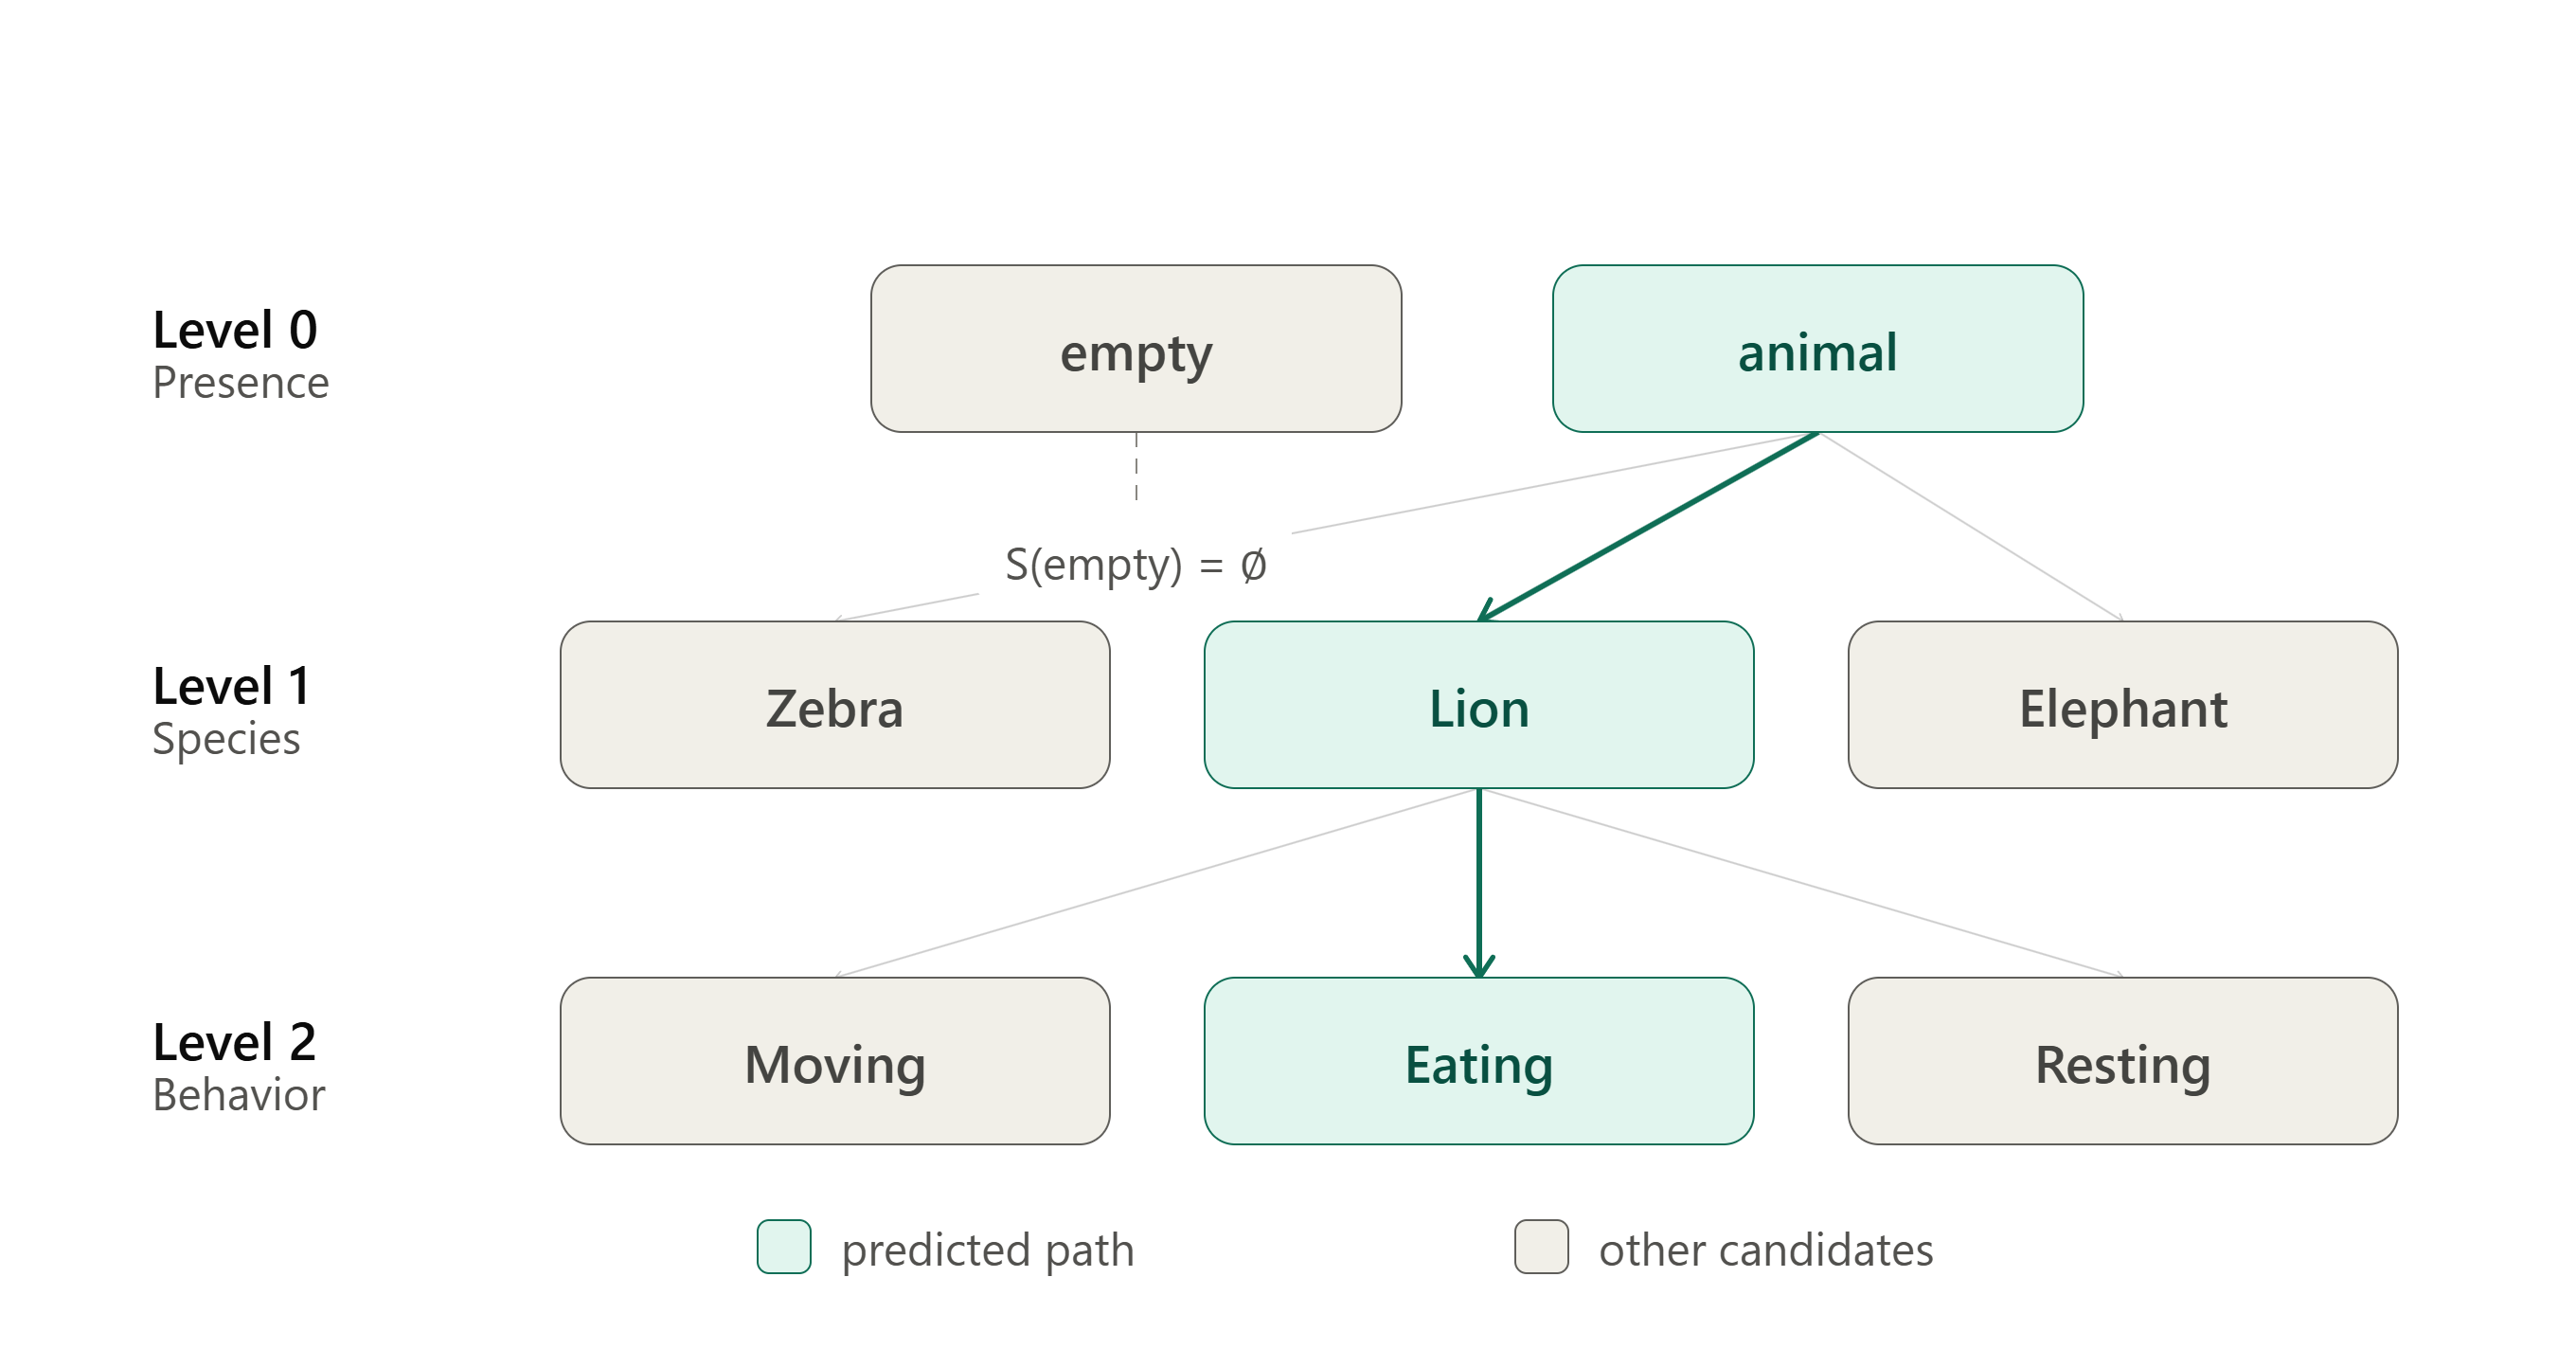
\includegraphics[width=6in]{images/eog_hierarchy_diagram.png}
\caption{The three-level Ecological Ontology Graph, illustrated with an example path. Level 0 separates presence (\textit{empty} vs.\ \textit{animal}); Level 1 conditions the species candidate set on the parent \textit{animal} node; Level 2 conditions the behavior candidate set on the parent species node. The highlighted path (\textit{animal} $\rightarrow$ \textit{lion} $\rightarrow$ \textit{eating}) illustrates one hierarchical prediction $(\hat{y}_0, \hat{y}_1, \hat{y}_2)$; \textit{empty} is a leaf node, since $S(\text{empty})=\emptyset$.}
\label{fig:eog_hierarchy}
\end{figure*}

Every EOG node $c$ at level $\ell$ is embedded through the same frozen text encoder and a level-specific trainable projection head into an embedding $e_c$ in the shared latent space. This is the mechanism that unifies the three tasks: instead of three separate classifiers, WildBind performs the same operation---similarity scoring against a set of candidate node embeddings---at each level of one hierarchy, with the candidate set at each level conditioned on the decision made at the level above.

\subsection{Contrastive Binding and Self-Supervised Pretraining}
\label{sec:contrastive_binding}

The central mechanism used to align the heterogeneous evidence sources in
WildBind is contrastive binding. Rather than requiring the different
modalities to share the same encoder, each modality is independently
projected into a common latent space. The visual event embedding serves as
the anchor representation, while the corresponding sequence, generated
description, ecological knowledge, and spatiotemporal context embeddings
provide complementary representations of the same camera-trap event.

For a given event $i$, the visual embedding $e_v^i$ and the corresponding
modality embedding $e_m^i$ form a positive pair. In contrast, modality
embeddings associated with other events in the same minibatch form negative
pairs. The contrastive objective therefore encourages representations
associated with the same event to become close in the shared latent space,
while separating representations originating from different events.
Figure~\ref{fig:contrastive_binding} illustrates the construction of positive
and negative pairs, the resulting similarity matrix, and the aggregation of
the modality-specific contrastive losses.

\begin{figure*}[!ht]
\centering
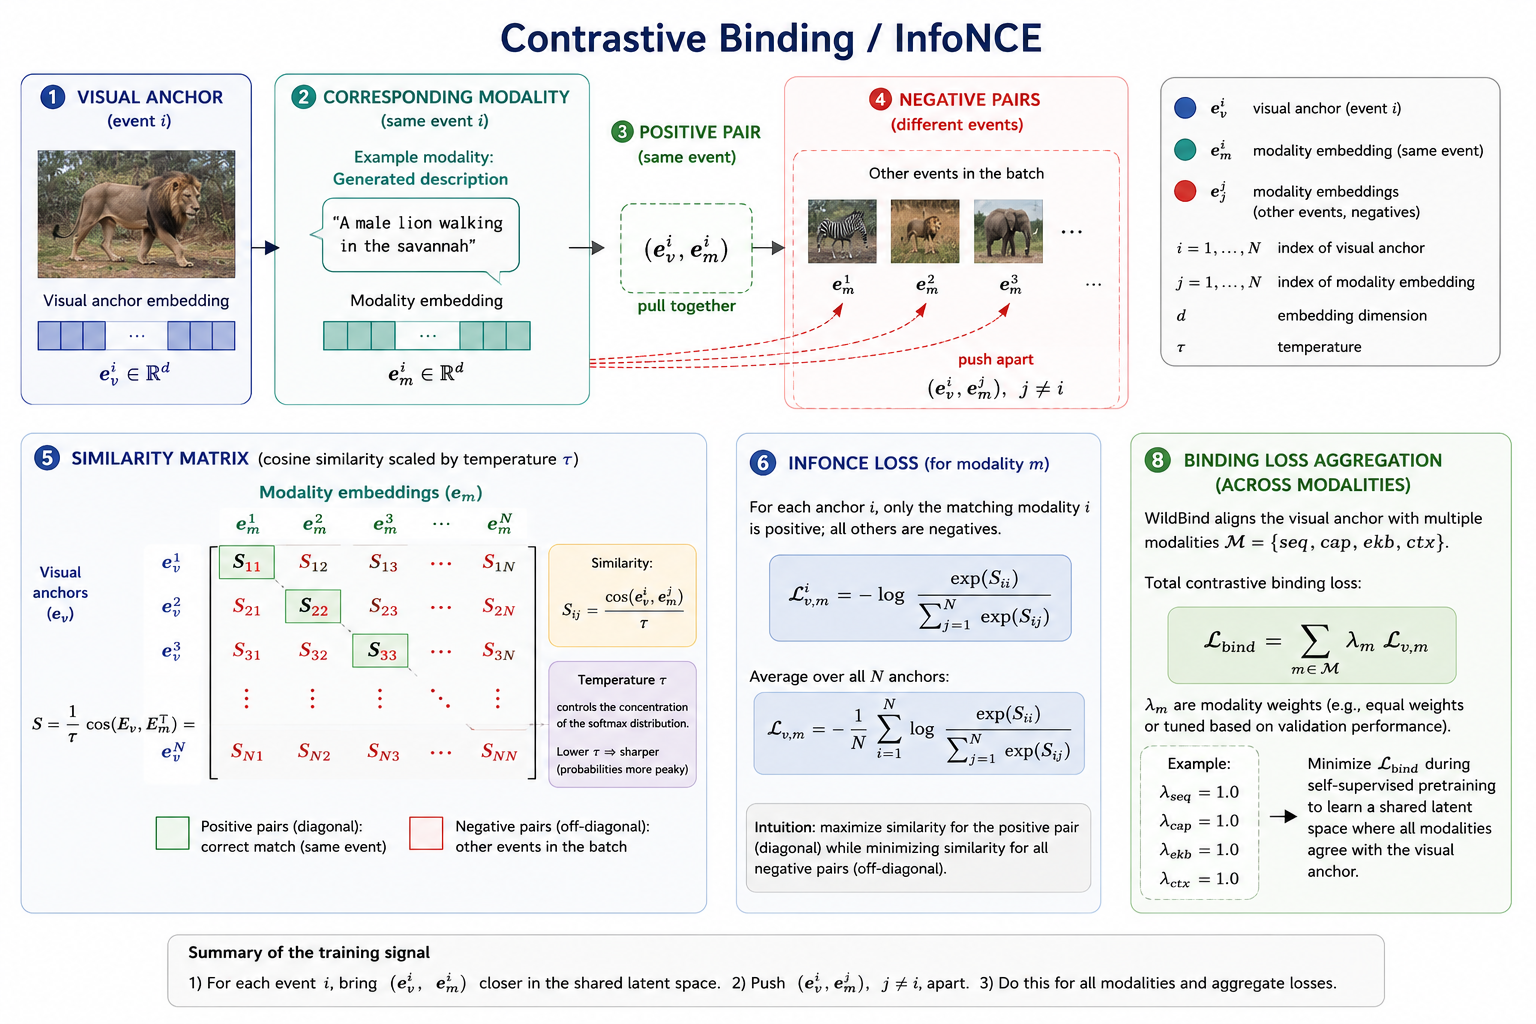
\includegraphics[width=6.5in]{images/contrastive_binding_infonce.png}
\caption{Illustration of the contrastive binding objective used in WildBind. For each camera-trap event $i$, the visual anchor embedding $e_v^i$ is paired with the embedding $e_m^i$ of the corresponding modality, forming a positive pair. Embeddings from different events in the minibatch form negative pairs. The temperature-scaled cosine similarities define the similarity matrix used by the InfoNCE objective. For each modality $m$, the contrastive loss $\mathcal{L}_{v,m}$ encourages the corresponding visual--modality pair to have high similarity while separating mismatched pairs. The individual modality losses are subsequently aggregated into the multimodal binding loss $\mathcal{L}_{bind}$.}
\label{fig:contrastive_binding}
\end{figure*}

For each visual--modality pair, the similarity between the visual anchor and
a modality embedding is computed using temperature-scaled cosine similarity:

\begin{equation}
S_{ij}^{(m)}
=
\frac{
\cos\left(e_v^i,e_m^j\right)
}{\tau},
\label{eq:similarity_temperature}
\end{equation}

where $e_v^i$ denotes the visual anchor embedding of event $i$,
$e_m^j$ denotes the embedding of modality $m$ associated with event $j$,
and $\tau$ is a learnable temperature parameter controlling the sharpness
of the similarity distribution.

For a minibatch containing $N$ events, the InfoNCE objective for modality
$m$ is defined as:

\begin{equation}
\mathcal{L}_{v,m}
=
-\frac{1}{N}
\sum_{i=1}^{N}
\log
\frac{
\exp\left(S_{ii}^{(m)}\right)
}{
\sum_{j=1}^{N}
\exp\left(S_{ij}^{(m)}\right)
}.
\label{eq:infonce}
\end{equation}

The numerator corresponds to the positive pair associated with the same
camera-trap event, whereas the denominator contains the positive pair and
all mismatched modality embeddings in the minibatch. Minimizing
$\mathcal{L}_{v,m}$ therefore increases the relative similarity between
matched visual--modality representations while reducing the similarity
between representations originating from different events.

The binding objective is applied independently to each peripheral modality
and subsequently aggregated into a single multimodal objective:

\begin{equation}
\mathcal{L}_{bind}
=
\sum_{m\in\mathcal{M}}
\lambda_m\mathcal{L}_{v,m},
\label{eq:binding_loss}
\end{equation}

where
$\mathcal{M}=\{\mathrm{seq},\mathrm{cap},\mathrm{ekb},\mathrm{ctx}\}$
denotes the set of peripheral modalities and $\lambda_m$ controls the
contribution of each modality to the overall binding objective. This
objective encourages the visual anchor to remain consistently aligned with
the heterogeneous evidence sources while preserving a shared latent
representation that can subsequently be used by the uncertainty-aware
fusion mechanism.

\subsection{Zero-Shot Inference and the Fusion Gate}\label{sec:fusion_gate}

At inference time, each available modality $m$ (including the visual anchor) produces its own similarity score against every EOG node $c$ under consideration at the current hierarchy level:

$$s_c^{(m)} = \cos\!\left(e_m,\, e_c^{(m)}\right)$$

where $e_c^{(m)}$ denotes the node embedding produced by the modality-specific projection head. This generalizes the two-branch score $f_s=\alpha \hat v_s+(1-\alpha)\hat t_s$ of Chapter~\ref{cap:experiment_02} (Equation therein) to an arbitrary number of modalities. Rather than a fixed $\alpha$, the modality weights are produced by a lightweight gating network $g_\theta$:

$$w = \mathrm{softmax}\Big(g_\theta\big([\,u\,;\,a\,]\big)\Big), \qquad f_c = \sum_{m \in \mathcal{M}\cup\{v\}} w_m \cdot a_m \cdot \hat{s}_c^{(m)}$$

where $u$ is a vector of per-modality uncertainty statistics (probability margin and normalized entropy of the modality's own ranking, computed directly from the similarity scores $s_c^{(m)}$), $a \in \{0,1\}^{|\mathcal{M}|+1}$ is a binary modality-availability mask, and $\hat{s}_c^{(m)}$ denotes the min--max normalized score. The gate $g_\theta$ is a two-layer MLP trained with cross-entropy against the ground-truth EOG node at each level, using only the small labeled validation partitions already available from Chapters~\ref{cap:experiment_01} and~\ref{cap:experiment_02}. The base encoders and projection heads remain frozen during this step, so training the gate is closer in cost to calibrating a handful of hyperparameters than to fine-tuning a foundation model. When a modality is unavailable, $a_m=0$ removes it from both the softmax and the weighted sum, so predictions degrade gracefully rather than failing, directly addressing the missing-modality limitation of fixed, two-branch fusion strategies discussed in the Motivation above.

Prediction proceeds hierarchically:

$$\hat{y}_0 = \arg\max_{c \in \{\text{empty},\,\text{animal}\}} f_c, \qquad
\hat{y}_1 = \arg\max_{c \in S(\hat{y}_0)} f_c, \qquad
\hat{y}_2 = \arg\max_{c \in B(\hat{y}_1)} f_c$$

where $S(\cdot)$ and $B(\cdot)$ denote the species and behavior candidate sets conditioned on the decision at the level above ($S(\text{empty})=\emptyset$, so the pipeline stops at Level 0 for images predicted empty). No parameters of the base visual or textual encoders are updated at any point, preserving a strict zero-shot regime with respect to the classes and events themselves, in the same sense used in Chapter~\ref{cap:experiment_02}.

\subsection{Implementation Plan}\label{sec:implementation_plan}

Realizing WildBind requires four categories of engineering work. The first is data handling shared with the earlier chapters: parsing event-level metadata, loading the ecological knowledge-base text, and applying MegaDetector to select, for each event, the frame and crop containing the highest-confidence animal detection, following the same detection step already used for filtering in Chapter~\ref{cap:experiment_01}. The second is the set of projection heads and the contrastive binding objective described in Section~\ref{sec:contrastive_binding}, which have no counterpart in Chapters~\ref{cap:experiment_01} or~\ref{cap:experiment_02} and constitute the core new component of WildBind. The third is the Ecological Ontology Graph itself, including the newly authored Behavior Knowledge Base, extending the species knowledge base already curated in Chapter~\ref{cap:experiment_02} to the presence and behavior levels. The fourth is the learned fusion gate $g_\theta$ (Section~\ref{sec:fusion_gate}), trained on the small labeled validation partitions already available from Chapters~\ref{cap:experiment_01} and~\ref{cap:experiment_02}. Native support for an arbitrary, possibly incomplete, subset of modalities at inference time is built into the gate from the start, so the four ablation configurations of Section~\ref{sec:eval_ablations} (visual-only, visual+burst, visual+context, and full) are simply four operating points of the same trained model, obtained by toggling the availability mask $a$, rather than four separate pipelines.

\section{Planned Experimental Evaluation}

\subsection{Datasets}

The evaluation reuses the datasets already curated for this thesis and adds one held-out dataset never used during pretraining or gate calibration, to test genuine cross-domain zero-shot generalization rather than in-distribution fusion gains:

\begin{itemize}
\item \textbf{Snapshot Serengeti} (seasons 1--6, Chapter~\ref{cap:experiment_01} splits) for empty-image filtering, species classification, and behavior identification, and the Serengeti subset used in Chapter~\ref{cap:experiment_02} for species classification with full-frame and cropped settings.
\item \textbf{Caltech Camera Traps and WCS} (Chapter~\ref{cap:experiment_02} subsets), reused for species classification and, subject to available annotation, for empty-image filtering.
\item \textbf{One fully held-out dataset} (candidates: ENA24-detection or the Wellington Camera Traps dataset), used exclusively at test time and excluded from contrastive pretraining and from gate calibration, to measure the accuracy gap between in-distribution and genuinely unseen deployments.
\end{itemize}

\subsection{Baselines and Ablations}\label{sec:eval_ablations}

Table~\ref{tab:wildbind_baselines} summarizes the planned comparison set.

\begin{table}[htbp]
\centering
\small
\caption{Planned baselines and ablations for the evaluation of WildBind.}
\label{tab:wildbind_baselines}
\begin{tabular}{p{3.6cm}p{4.2cm}p{4.9cm}}
\toprule
\textbf{Configuration} & \textbf{Modalities used} & \textbf{Purpose} \\
\midrule
Task-specific zero-shot models (CLIP, BLIP, GPT, Gemini) & Single modality, single task & Reuse of Chapter~\ref{cap:experiment_01} results as task-specific lower/upper reference points. \\
WildMatch-VLM-Fusion & Visual + generated description, fixed $\alpha$ & Reuse of Chapter~\ref{cap:experiment_02} results; isolates the benefit of a \emph{learned} gate over a fixed weight, on the species-classification task alone. \\
WildBind -- visual only & $e_v$ & Lower bound relying solely on the visual anchor, with no peripheral modality contributing to the fused score. \\
WildBind -- visual + burst & $e_v, e_{seq}$ & Isolates the contribution of burst-level temporal context over the single-frame anchor. \\
WildBind -- visual + context & $e_v, e_{ekb}, e_{ctx}$ & Isolates the contribution of ecological-knowledge and spatiotemporal-metadata evidence, without generated captions. \\
WildBind -- full & $e_v, e_{seq}, e_{cap}, e_{ekb}, e_{ctx}$ & Main proposed configuration, combining all five evidence sources through the learned gate. \\
WildBind -- fixed-weight gate & Same as full, $w$ fixed instead of learned & Ablation isolating the contribution of the learned gate itself. \\
Supervised instruction-tuned reference & Full fine-tuning of an open VLM (e.g., Qwen2.5-VL or LLaVA) in the spirit of CameraTrap-Instruct & Upper-bound reference quantifying the accuracy/supervision-cost trade-off relative to a fully supervised, non-zero-shot unified model. \\
\bottomrule
\end{tabular}
\end{table}

\subsection{Evaluation Metrics}

Consistent with Chapters~\ref{cap:experiment_01} and~\ref{cap:experiment_02}, the evaluation reports top-1 and top-$k$ accuracy, macro F1-score, and balanced accuracy per task and per dataset, together with 95\% confidence intervals. Three metrics specific to the unified design are added:

\begin{itemize}
\item \textbf{Chain accuracy}: the proportion of events for which presence, species, and (when applicable) behavior are \emph{all} predicted correctly, quantifying the cost of hierarchical error propagation that a task-unified model uniquely exposes.
\item \textbf{Missing-modality robustness curve}: accuracy as a function of the number of available peripheral modalities ($|a|_1 = 0, 1, \dots, 4$), analogous to the coverage analysis reported for FunBind \citep{boadu2025funbind}, quantifying graceful degradation.
\item \textbf{Cross-domain generalization gap}: the accuracy difference between the in-distribution test partitions and the held-out dataset, isolating genuine zero-shot transfer from in-distribution fusion gains.
\end{itemize}

\subsection{Statistical Analysis Plan}

Aggregate accuracy differences across configurations and datasets will be assessed with the Friedman test, followed by Nemenyi post-hoc pairwise comparisons, mirroring the protocol used in Chapter~\ref{cap:experiment_02}. Paired classification agreement between WildBind and the two closest competitors (WildMatch-VLM-Fusion and the supervised instruction-tuned reference) will additionally be tested with McNemar's test on the presence/absence and species-classification decisions, and bootstrap resampling (1{,}000 resamples) will be used to obtain confidence intervals for the chain-accuracy metric, which has no standard closed-form variance estimator.

\subsection{Expected Outcomes and Risks}

Three outcomes are anticipated, framed as testable extensions of Hypotheses H1--H3 (Chapter~\ref{cap:introduction}): (i) a learned, uncertainty-aware gate should outperform both the visual-only baseline and the fixed-$\alpha$ fusion of Chapter~\ref{cap:experiment_02} on species classification, since it can adapt its reliance on textual evidence per instance rather than globally; (ii) task unification through the Ecological Ontology Graph should reduce the variance in effectiveness across tasks observed in Chapter~\ref{cap:experiment_01}, since presence, species, and behavior share the same embedding space and calibration procedure; (iii) the accuracy gap between WildBind and the supervised instruction-tuned reference is expected to be non-zero, and reporting it honestly is itself a contribution, since it quantifies the price of remaining in a low-supervision regime. The main anticipated risk is that behavior-level textual descriptions (the newly required Behavior Knowledge Base) may be substantially harder to author at a useful level of visual specificity than species descriptions were in Chapter~\ref{cap:experiment_02}, given that behavior is posture- and context-dependent rather than morphological; this risk will be mitigated by reusing the sequence-based visual evidence ($e_{seq}$) as the dominant signal for behavior, with the Behavior Knowledge Base acting only as a secondary re-ranking signal, mirroring the comparatively lower weight ($1-\alpha=0.3$) already given to textual evidence relative to the visual signal in Chapter~\ref{cap:experiment_02}.

\section{Discussion: Positioning and Limitations}

WildBind is deliberately scoped as a methodological and architectural contribution rather than a claim of universal superiority. Three limitations should be acknowledged from the outset of the proposal. First, the learned gate, however lightweight, reintroduces a small amount of task-specific supervision that the purely zero-shot components of this thesis (Chapters~\ref{cap:experiment_01} and~\ref{cap:experiment_02}) avoided. This is a deliberate trade-off, justified by the expectation that a few hundred labeled calibration events are sufficient to train a two-layer gate, several orders of magnitude less than the data required to instruction-tune a vision-language model. Second, the Ecological Ontology Graph assumes a closed candidate set at each level, so genuinely novel species or behaviors still require adding a textual description to the corresponding knowledge base, a limitation shared with WildMatch-VLM-Fusion and with the sequence-anchored zero-shot mode of FunBind. Third, the reliance on MegaDetector for keyframe and crop selection inherits any systematic detection failures of that model. This dependency is carried over from the same detection pipeline already used in Chapter~\ref{cap:experiment_01} and is treated here as an explicit design choice rather than an oversight.

\section{Final Remarks}

This chapter proposed WildBind, a unified multimodal binding architecture for camera-trap understanding that treats empty-image filtering, species classification, and behavior identification as one hierarchical retrieval problem over a shared Ecological Ontology Graph, and that fuses an arbitrary number of visual, sequence, textual, and contextual evidence sources through a learned, uncertainty-aware gate rather than a fixed weight. The design is directly inspired by, and explicitly differentiated from, a structurally similar unified multimodal binding model recently proposed for protein function prediction \citep{boadu2025funbind}, and is positioned against CameraTrap-Instruct \citep{chen2026cameratrap} as a lower-supervision alternative that keeps its backbones frozen. The architecture is specified in enough detail to be implemented directly, with the required data-loading, keyframe-selection, ontology, and gate-training components laid out in Section~\ref{sec:implementation_plan}. The bulk of the new development effort is concentrated in the projection heads, the contrastive binding objective, the Ecological Ontology Graph (including a new Behavior Knowledge Base), and the learned fusion gate. Within the context of this thesis, this chapter is intended to constitute the third and most conceptually integrative contribution: where Chapter~\ref{cap:experiment_01} characterized the instability of standalone multimodal inference and Chapter~\ref{cap:experiment_02} showed that a simple fixed fusion of two signals can partially address this instability for one task, this chapter proposes a single learned mechanism that generalizes both findings across all three camera-trap tasks studied in this thesis.